\section{Experiments and results}
\label{sec:experiments}

% In our experiments, we consider the two properties of systematicity (\S\ref{subsec:systematicity}) and substitutivity (\S\ref{subsec:substitutivity}), that require local meaning compositions, % traditionally associated with compositionality:
In our experiments, we consider \emph{systematicity} (\S\ref{subsec:systematicity}) and \emph{substitutivity} (\S\ref{subsec:substitutivity}), to test for local compositionality, % traditionally associated with compositionality:
and \emph{idiom translation} %-- traditionally considered problematic for the compositionality of natural language --
to probe for a more global type of processing (\S\ref{subsec:global_compositionality}).

\begin{figure*}[!ht]
    \centering
    \begin{subfigure}[b]{\columnwidth}
    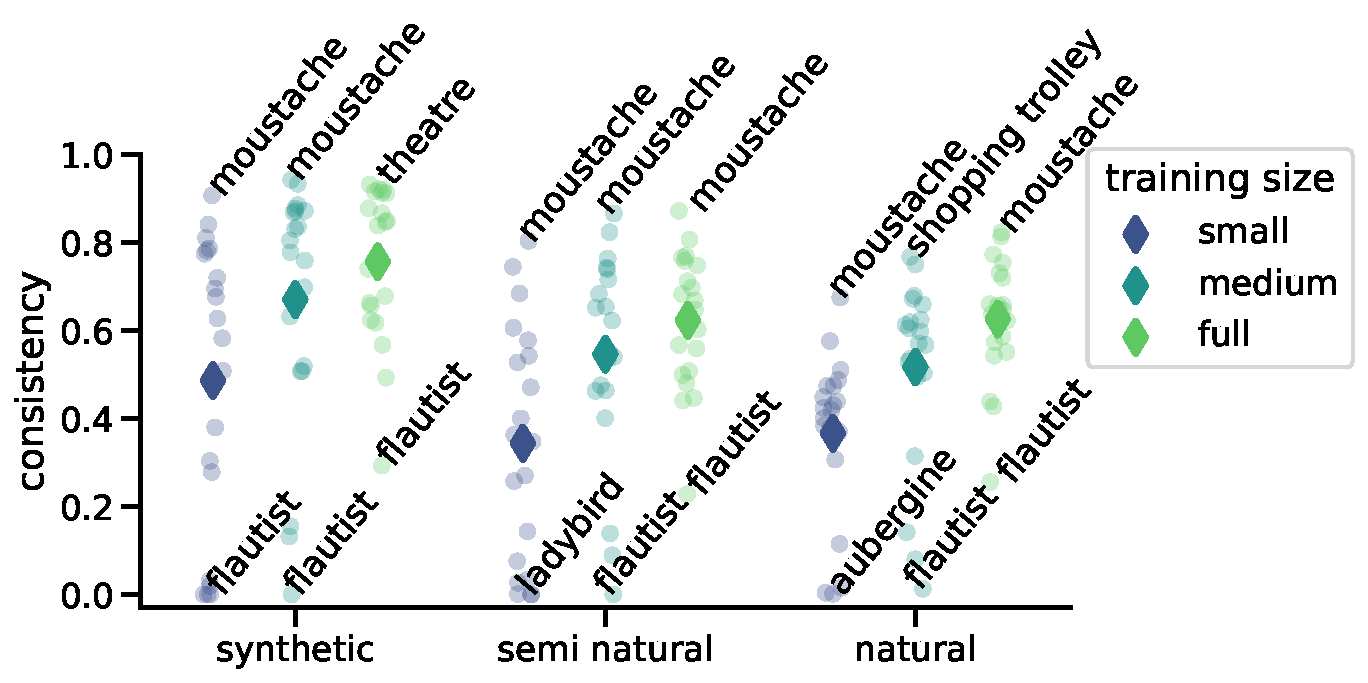
\includegraphics[width=\columnwidth]{figures/substitutivity/consistency.pdf}
    % \vspace{-0.3cm}
    \caption{}
        \vspace{-2mm}
    \label{fig:substitutivity}
    \end{subfigure}
% \end{figure}
% \begin{figure}
%V\centering
    \begin{subfigure}[b]{\columnwidth}
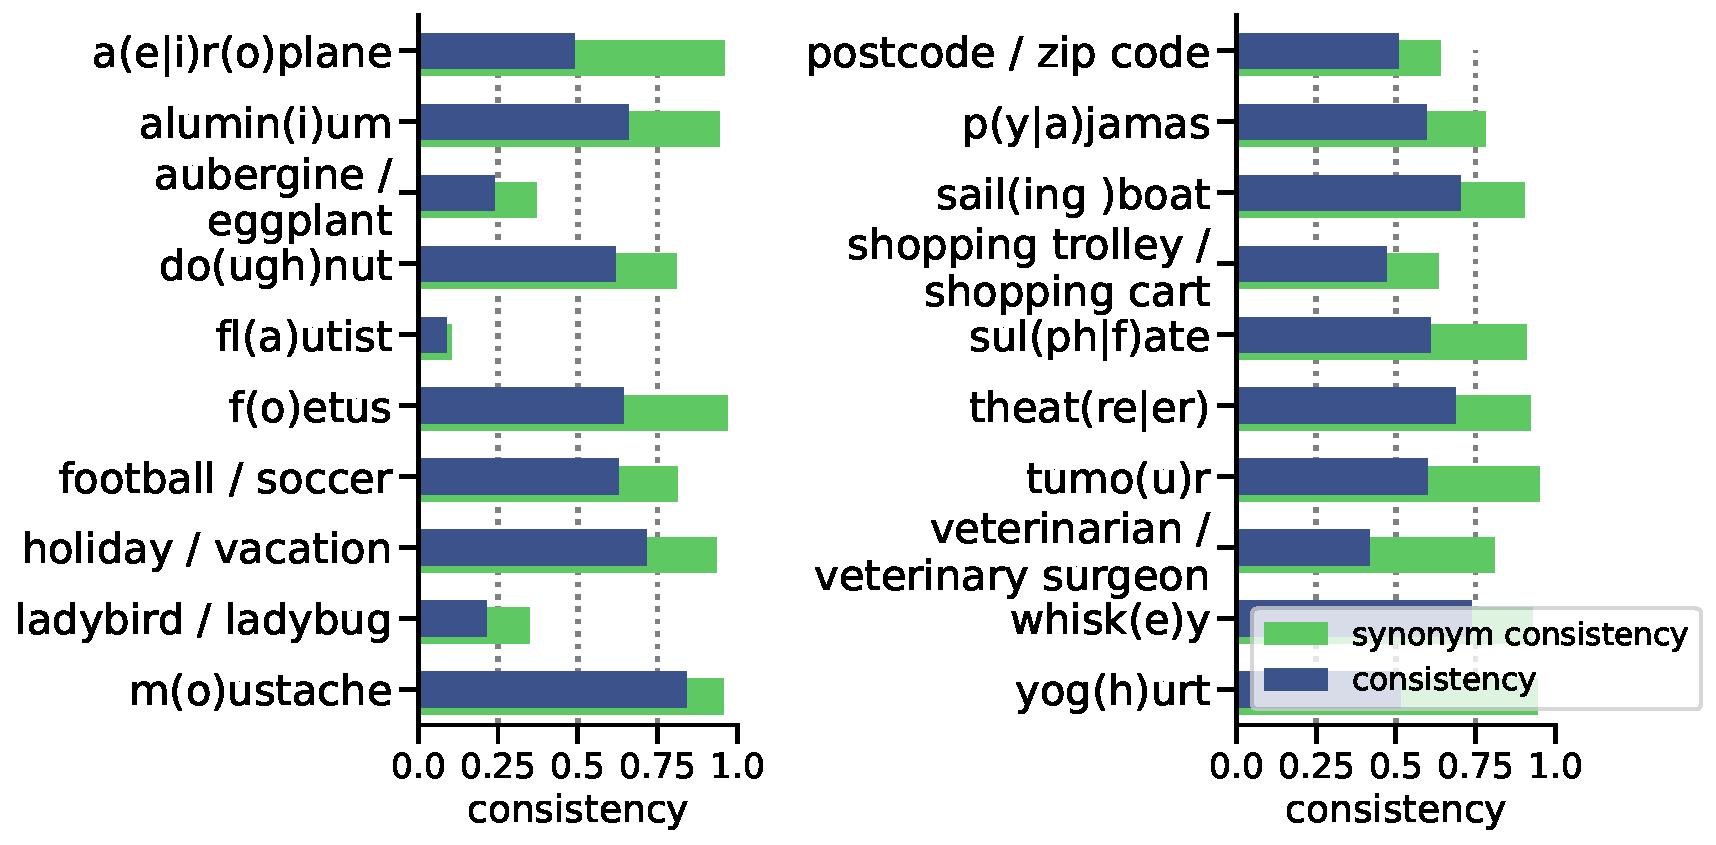
\includegraphics[width=\columnwidth]{figures/substitutivity/noun_consistency.pdf}
        \caption{}
        \vspace{-2mm}
\label{fig:per_synonym}
    \end{subfigure}
% \vspace{-0.3cm}
    \caption{(a) Consistency scores of synonyms (averaged $\diamond$, and per synonym $\circ$) for substitutivity per evaluation data type, for three training set sizes.
    %We annotate synonyms with the highest and lowest scores.
    (b) Consistency per synonym, measured using full sentences (in dark blue) or the synonym's translation only (in green), averaged over training dataset sizes and data types.}
    % \label{fig:substitutivity}
\vspace{-0.3cm}
\end{figure*}

\subsection{Systematicity}
\label{subsec:systematicity}

One of the most commonly tested properties of compositional generalisation is \textbf{systematicity} -- the ability to understand novel combinations made up from known components \citep[most famously,][]{lake2018generalization}.
In natural data, the number of potential recombinations to consider is infinite.
We chose to focus on recombinations in two sentence-level context-free rules: \texttt{S\;$\rightarrow$\;NP\;VP} and \texttt{S\;$\rightarrow$\;S\;CONJ\;S}.

\subsubsection{Experiments}
\paragraph{Test design}
\label{subsec:systematicity_test_design}
The first setup, \texttt{S\;$\rightarrow$\;NP\;VP}, concerns recombinations of noun and verb phrases.
We extract translations for input sentences from the templates from \S\ref{sec:data}, as well as versions of them with the (1) noun (NP $\rightarrow$ NP') or (2) verb phrase (VP $\rightarrow$ VP') adapted.
In (1), a noun from the NP in the subject position is replaced with a different noun while preserving number agreement with the VP.
In (2), a noun in the VP is replaced.
NP $\rightarrow$ NP' is applied to both synthetic and semi-natural data; VP $\rightarrow$ VP' only to synthetic data.
We use 500 samples per template per condition per data type.

The second setup, \texttt{S\;$\rightarrow$\;S\;CONJ\;S}, involves phrases concatenated using \exa{and}, and tests whether the translation of the second sentence is dependent on the first sentence.
We concatenate two sentences ($\text{S}_1$ and $\text{S}_2$) from different templates, and we consider again two different conditions.
First, in condition $\text{S}_1\rightarrow\text{S}^\prime_1$, we make a minimal change to $\text{S}_1$ yielding $\text{S}^\prime_1$ by changing the noun in its verb phrase.
In $\text{S}_1\rightarrow\text{S}_3$, instead, we replace $\text{S}_1$ with a sentence $\text{S}_3$ that is sampled from a template different from $\text{S}_1$.
We compare the translation of $\text{S}_2$ in all conditions.
For consistency, the first conjunct is always sampled from the synthetic data templates. 
The second conjunct is sampled from synthetic data, semi-natural data, or from natural sentences sampled from \textsc{OPUS} with similar lengths and word-frequencies as the semi-natural inputs.
We use 500 samples per template per condition per data type.
Figure~\ref{fig:systematicity_explanation} provides an illustration of the different setups experimented with.

\paragraph{Evaluation}
In artificial domains, systematicity is evaluated by leaving out combinations of `known components' from the training data and using them for testing purposes.
The necessary familiarity of the components (the fact that they are `known') is ensured by high training accuracies, and systematicity is quantified by measuring the test set accuracy.
If the training data is a natural corpus and the model is evaluated with a measure like BLEU in MT, this strategy is not available.
We observe that being systematic requires being consistent in the interpretation assigned to a (sub)expression across contexts, both in artificial and natural domains.
Here, we, therefore, focus on \textbf{consistency} rather than accuracy, allowing us to employ a model-driven approach that evaluates the model's systematicity as the consistency of the translations when presenting words or phrases in multiple contexts.

We measure consistency as the equality of two translations after accounting for anticipated changes.
For instance, in the \texttt{S\;$\rightarrow$\;NP\;VP} setup, two translations are consistent if they differ in one word only, after accounting for determiner changes in Dutch (\exa{de} vs\ \exa{het}).
In the evaluation of \texttt{S\;$\rightarrow$\;S\;CONJ\;S}, we measure the consistency of the translations of the second conjunct.

\subsubsection{Results}
Figure~\ref{fig:systematicity} shows the results for the \texttt{S\;$\rightarrow$\;NP\;VP} and \texttt{S\;$\rightarrow$\;S\;CONJ\;S} setups (numbers available in Appendix~\ref{ap:systematicity}).
The average performance for the natural data closely resembles the performance on \textit{semi-}natural data, suggesting that the increased degree of control did not severely impact the results obtained using this generated data.\footnote{In our manual analysis (\S\ref{sec:manual_analysis}), however, we did observe a slightly different distribution of changes between these setups.}
In general, the consistency scores are low, illustrating that models are prone to changing their translation of a (sub)sentence after small (unrelated) adaptations to the input.
It hardly matters whether that change occurs in the sentence itself (\texttt{S\;$\rightarrow$\;NP\;VP}), or in the other conjunct (\texttt{S\;$\rightarrow$} \texttt{S\;CONJ\;S}), suggesting that the processing of the models is not local as assumed in strong compositionality.
Models trained on more data seem more locally compositional, a somewhat contradictory solution to achieving compositionality, which, after all, is assumed to underlie the ability to generalise usage from \emph{few} examples \citep{lake2019human}.
This trend is also at odds with the hypothesis that inconsistencies are a consequence of the natural variation of language, which models trained on \emph{more} data are expected to better capture.


\subsection{Substitutivity}
\label{subsec:substitutivity}

Under a local interpretation of the principle of compositionality, synonym substitutions should be meaning-preserving: substituting a constituent in a complex expression with a synonym should not alter the complex expression's meaning, or, in the case of MT, its translation.
Here, we test to what extent models' translations abide by this principle, by performing the \textbf{substitutivity} test from \citet{hupkes2020compositionality}, that measures whether the outputs remain consistent after synonym substitution.

\subsubsection{Experiments}
To find synonyms -- source terms that translate into the same target terms -- we exploit the fact that OPUS contains texts both in British and American English.
Therefore, it contains synonymous terms that are spelt different -- e.g.\ \exa{doughnut} / \exa{donut} -- and synonymous terms with a very different form -- e.g.\ \exa{aubergine} / \exa{eggplant}.
We use 20 synonym pairs in total (see Figure~\ref{fig:per_synonym}).

\paragraph{Test design}
Per synonym pair, we select natural data from OPUS in which the terms appear and perform synonym substitutions.
Thus, each sample has two sentences, one with the British and one with the American English term.
We also insert the synonyms into the synthetic and semi-natural data using 500 samples per synonym pair per template, through subordinate clauses that modify a noun -- e.g. ``the king \textit{that eats the doughnut}''.
In Appendix~\ref{ap:substitutivity}, Table~\ref{tab:substitutivity_appendix}, we list all clauses used.

\paragraph{Evaluation}
Like systematicity, we evaluate substitutivity using the consistency score, expressing whether the model translations for a sample are identical.
We report both the full sentence consistency and the consistency of the synonyms' translations only, excluding the context.
Cases in which the model omits the synonym from both translations are labelled as consistent if the rest of the translation is the same for both input sequences.

\subsubsection{Results}
In Figure~\ref{fig:substitutivity}, we summarise all substitutivity consistency scores (tables are in Appendix~\ref{ap:substitutivity}).
We observe trends similar to the systematicity results: models trained on larger training sets perform better and synthetic data yields more consistent translations compared to (semi-)natural data.
We further observe large variations across synonyms, for which we further detail the performance aggregated across experimental setups in Figure~\ref{fig:per_synonym}.
The three lowest scoring synonyms -- \exa{flautist}, \exa{aubergine} and \exa{ladybug} -- are among the least frequent synonyms (see Appendix~\ref{ap:substitutivity}), which stresses the importance of frequency for the model to pick up on synonymy.

In Figure~\ref{fig:per_synonym}, we show both the regular consistency and the consistency of the synonym translations, illustrating that a substantial part of the inconsistencies are due to varying translations of the context rather than the synonym itself, stressing again the non-local processing of the models.

\subsection{Global compositionality}
\label{subsec:global_compositionality}

In our final test, we focus on exceptions to compositional rules.
In natural language, typical exceptions that constitute a challenge for local compositionality are \emph{idioms}.
For instance, the idiom ``raining cats and dogs'' should be treated globally to arrive at its meaning of heavy rainfall.
A local approach would yield an overly literal, non-sensical translation (``het regent katten en honden'').
When a model's translation is too local, we follow \citet{hupkes2020compositionality} in saying that it \textbf{overgeneralises}, or, in other words, it applies a general rule to an expression that is an exception to this rule.
Overgeneralisation indicates that a language learner has internalised the general rule \citep[e.g.][]{penke2012dual}.

\subsubsection{Experiments}
We select 20 English idioms for which an accurate Dutch translation differs from the literal translation from the English MAGPIE corpus \citep{haagsma2020magpie}.
Because acquisition of idioms is dependent on their frequency in the corpus, we use idioms with at least 200 occurrences in OPUS based on exact matches, for which over 80\% of the target translations does not contain a literal translation.

\paragraph{Test design}
Per idiom, we extract \textit{natural} sentences containing the idiom from OPUS. 
For the synthetic and semi-natural data types, we insert the idiom in 500 samples per idiom per template, by attaching a subordinate clause to a noun -- e.g.\ ``the king \emph{that said `I knew the formula \textbf{by heart}'}''. 
The clauses used can be found in Appendix~\ref{ap:global_compositionality}, Table~\ref{tab:overgeneralisation_appendix}.

\paragraph{Evaluation}
Per idiom, we assess how often a model overgeneralises and how often it translates the idiom globally. 
To do so, we identify keywords that indicate that a translation is translated locally (literal) instead of globally (idiomatic).
If the keywords' literal translations are present, the translation is labelled as an overgeneralised translation. 
For instance, for ``by heart'', the presence of ``hart'' (``heart'') suggests a literal translation. An adequate paraphrase would say ``uit het hoofd'' (``from the head'').
See Appendix~\ref{ap:global_compositionality}, Table~\ref{tab:overgeneralisation_appendix}, for the full list of keywords.
We evaluate overgeneralisation for ten intermediate training checkpoints.

\begin{figure}
    \centering
    \begin{subfigure}[b]{\columnwidth}\centering
    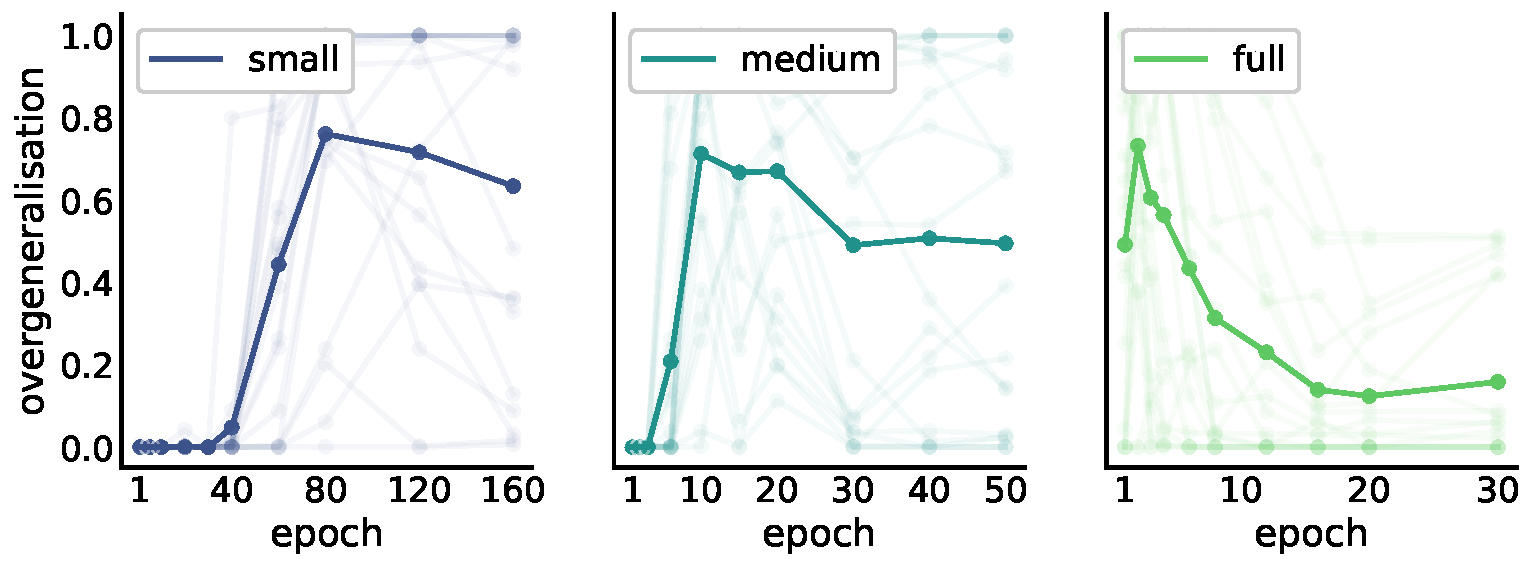
\includegraphics[width=\textwidth]{figures/global_compositionality/synthetic.pdf}
    \caption{Synthetic}
    \end{subfigure}
    \begin{subfigure}[b]{\columnwidth}\centering
    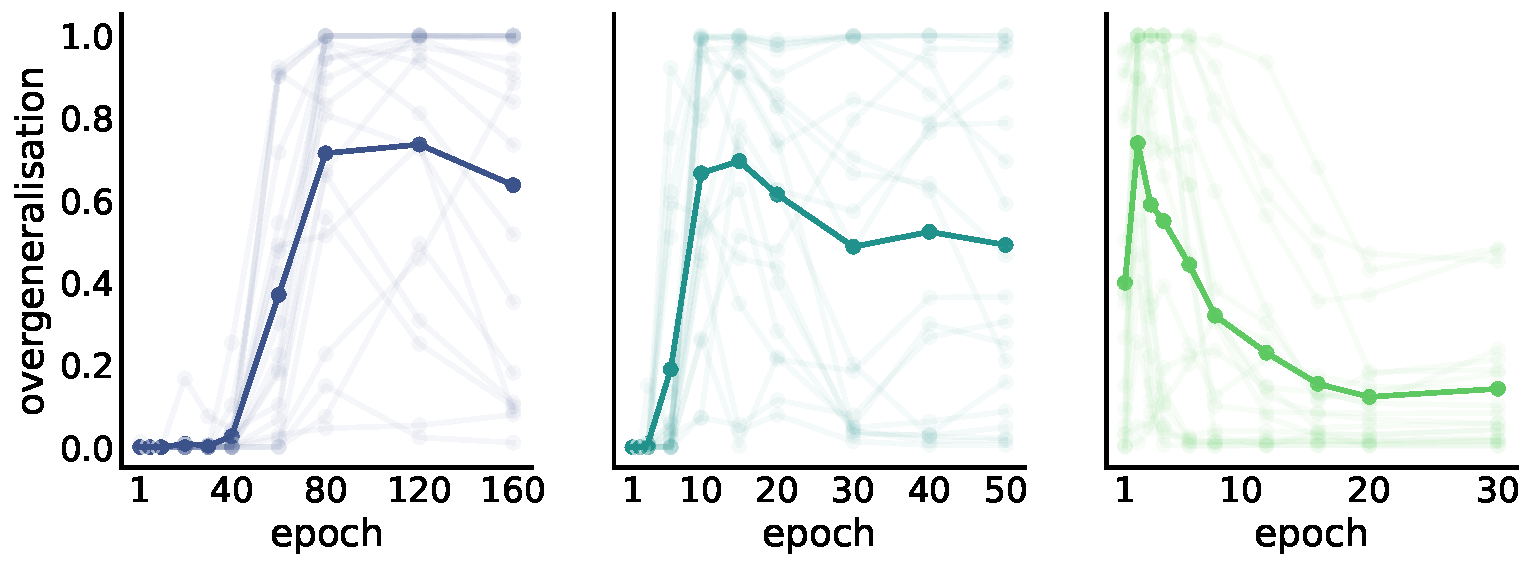
\includegraphics[width=\textwidth]{figures/global_compositionality/semi_natural.pdf}
    \caption{Semi-Natural}
    \end{subfigure}
    \begin{subfigure}[b]{\columnwidth}\centering
    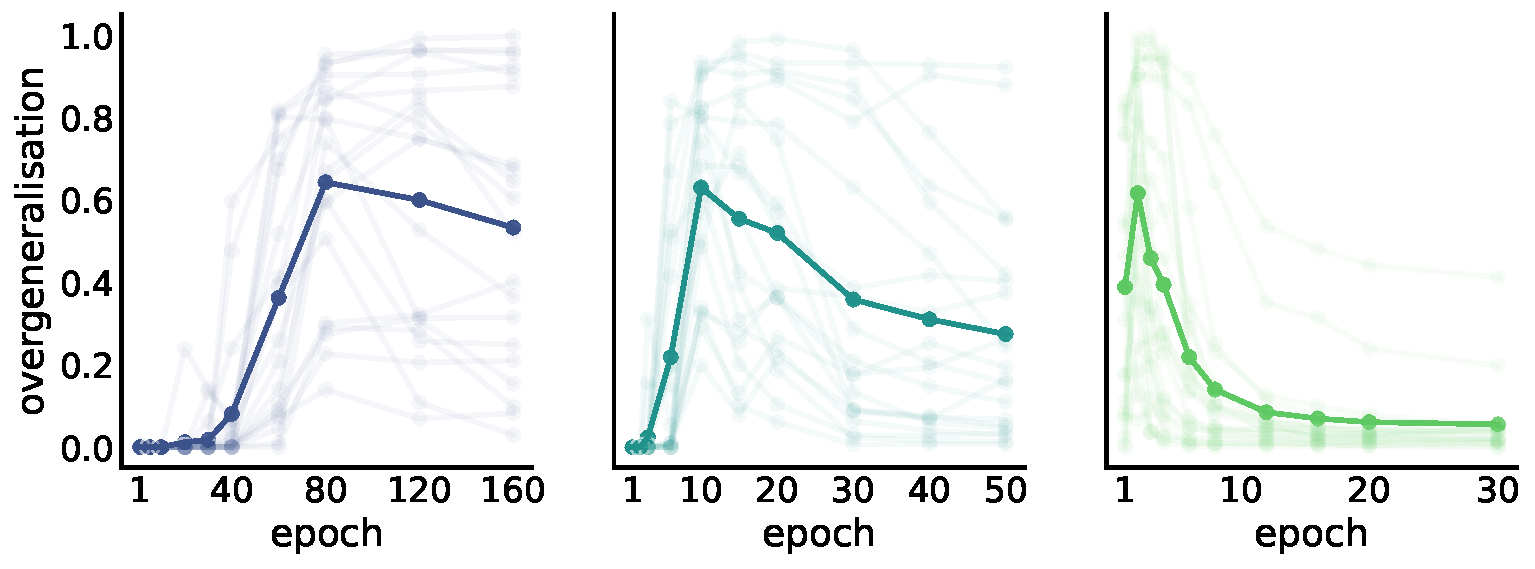
\includegraphics[width=\textwidth]{figures/global_compositionality/natural.pdf}
    \caption{Natural}
    \end{subfigure}
    \caption{Visualisation of overgeneralisation for idioms throughout training, with a line per idiom and the overall mean. Overgeneralisation occurs early on in training and precedes memorisation of idioms' translations.
    The colours indicate different training dataset sizes.}
    \label{fig:global_compositionality}
    \vspace{-0.3cm}
\end{figure}

\subsubsection{Results}
In Figure~\ref{fig:global_compositionality}, we report our results.\footnote{Note that epochs consist of different numbers of samples: 1M, 8.6M and 69M for small, medium and full. Appendix~\ref{ap:global_compositionality} further details numerical results per idiom.}
For all evaluation data types and all training set sizes, three phases can be identified.
Initially, the translations do not contain the idiom's keyword, not because the idiom's meaning is paraphrased in the translation, but because the translations consist of high-frequency words in the target language only. 
Afterwards, overgeneralisation peaks: the model emits a very literal translation of the idiom.
Finally, the model starts to memorise the idiom's translation.
This is in accordance with results from \citet{hupkes2020compositionality}, and earlier results presented in the past tense debate by -- among others -- \citet{rumelhart1986learning}.

Although the height of the overgeneralisation peak is similar across evaluation data types and training set sizes, overgeneralisation is more prominent in converged models trained on smaller datasets than it is in models trained on the full corpus.\footnote{Convergence is based on BLEU scores for validation data.}
In addition to training dataset size, the type of evaluation data used also matters: there is more overgeneralisation for synthetic and semi-natural data compared to natural data, stressing the impact of the context in which an idiom is embedded.
The extreme case of a context unsupportive of an idiomatic interpretation is a sequence of random words. To evaluate the hypothesis that this yields local translations, we surround the idioms with ten random words.
The results (Appendix~\ref{ap:global_compositionality}, Table~\ref{tab:overgeneralisation_appendix}) indicate that, indeed,  when the context provides no support at all for a global interpretation, the model provides a local translation for nearly all idioms.
Overall, the results of this test provide an interesting contrast with our substitutivity and systematicity results: where in those tests, we saw processing that was \emph{less local} than we expected, here, the behaviour shown by the models is instead \emph{not global enough}.
